%%%%%%%%%%%%%%%%%%%%%%%%%%%%%%%%%%%%%%%%%%%%%%%
%
% Template per Elaborato di Laurea
% DISI - Dipartimento di Ingegneria e Scienza dell’Informazione
%
% update 2015-09-10
%
% Per la generazione corretta del 
% pdflatex nome_file.tex
% bibtex nome_file.aux
% pdflatex nome_file.tex
% pdflatex nome_file.tex
%
%%%%%%%%%%%%%%%%%%%%%%%%%%%%%%%%%%%%%%%%%%%%%%%

% formato FRONTE RETRO
\documentclass[epsfig,a4paper,11pt,titlepage,twoside,openany]{book}
\usepackage{epsfig}
\usepackage{plain}
\usepackage{setspace}
\usepackage[paperheight=29.7cm,paperwidth=21cm,outer=1.5cm,inner=2.5cm,top=2cm,bottom=2cm]{geometry} % per definizione layout
\usepackage{titlesec} % per formato custom dei titoli dei capitoli

%%%%%%%%%%%%%%
% supporto lettere accentate
%
%\usepackage[latin1]{inputenc} % per Windows;
\usepackage[utf8x]{inputenc} % per Linux (richiede il pacchetto unicode);
%\usepackage[applemac]{inputenc} % per Mac.

% supporto simboli matematici
\usepackage{amsfonts}
\usepackage{amsmath}
\usepackage{multirow}
\usepackage{caption}

\usepackage{amssymb}
\usepackage{graphicx}

\usepackage{url}									
\usepackage{hyperref}

\singlespacing

\usepackage[english]{babel}

\newcommand{\emptypage}{
        \newpage
        %\thispagestyle{empty}
        \mbox{}
        \newpage
        %\addtocounter{page}{-1}
        }

\begin{document}

  % nessuna numerazione
  \pagenumbering{gobble} 
  \pagestyle{plain}

\thispagestyle{empty}

\begin{center}
  \begin{figure}[h!]
    \centerline{
\psfig{file=marchio_unitrento_colore_it_202002.eps,width=0.6\textwidth}}
  \end{figure}

  \vspace{2 cm} 

  \LARGE{Department of Information Engineering and Computer Science\\}

  \vspace{1 cm} 
  \Large{Bachelor's Degree in\\
    Computer, Communication and Electronic Engineering}

  \vspace{2 cm} 
  \Large\textsc{Final dissertation\\} 
  \vspace{1 cm} 
  \Huge\textsc{Backpropagation-based reinforcement learning for decision trees\\}



  \vspace{2 cm} 
  \begin{tabular*}{\textwidth}{ c @{\extracolsep{\fill}} c }
  \Large{Supervisor} & \Large{Student}\\
  \Large{Prof. IACCA Giovanni}& \Large{SCEVAROLI Simone}\\
  &\\
  \Large{Co-supervisor}&\\
  \Large{CUSTODE Leonardo Lucio}\\
  \end{tabular*}

  \vspace{2 cm} 

  \Large{Academic year 2021/2022}
  
\end{center}



  \clearpage
  \emptypage
  
 
%%%%%%%%%%%%%%%%%%%%%%%%%%%%%%%%%%%%%%%%%%%%%%%%%%%%%%%%%%%%%%%%%%%%%%%%%%
%%%%%%%%%%%%%%%%%%%%%%%%%%%%%%%%%%%%%%%%%%%%%%%%%%%%%%%%%%%%%%%%%%%%%%%%%%
%% Nota
%%%%%%%%%%%%%%%%%%%%%%%%%%%%%%%%%%%%%%%%%%%%%%%%%%%%%%%%%%%%%%%%%%%%%%%%%%
%% Sezione Ringraziamenti opzionale
%%%%%%%%%%%%%%%%%%%%%%%%%%%%%%%%%%%%%%%%%%%%%%%%%%%%%%%%%%%%%%%%%%%%%%%%%%
%%%%%%%%%%%%%%%%%%%%%%%%%%%%%%%%%%%%%%%%%%%%%%%%%%%%%%%%%%%%%%%%%%%%%%%%%%
  \thispagestyle{empty}

\begin{center}
  {\bf \Huge Acknowledgements}
\end{center}

\vspace{4cm}


\emph{\\I would like to express my deepest appreciation to professor Iacca for giving me the opportunity to do this work of thesis under his supervision. He is always available in the need and his truly passion for his subject gave me a strong motivation to carry out my research.\\I’m extremely grateful to Leonardo and Andrea for helping me in the technical part of this work, despite their many academic commitments.\\Thanks to my family, that always supports me in every choice of my life and never made me miss anything.\\A special thanks to my girlfriend Elisa, who for three years gave me the strength to bring out the very best of me in every situation, staying with me in the most difficult moments and sharing with me the aspirations and dreams for the future.
}

  \clearpage
  \emptypage
  \pagestyle{plain} % nessuna intestazione e pie pagina con numero al centro

  
  % inizio numerazione pagine in numeri arabi
  \mainmatter

%%%%%%%%%%%%%%%%%%%%%%%%%%%%%%%%%%%%%%%%%%%%%%%%%%%%%%%%%%%%%%%%%%%%%%%%%%
%%%%%%%%%%%%%%%%%%%%%%%%%%%%%%%%%%%%%%%%%%%%%%%%%%%%%%%%%%%%%%%%%%%%%%%%%%
%% Nota
%%%%%%%%%%%%%%%%%%%%%%%%%%%%%%%%%%%%%%%%%%%%%%%%%%%%%%%%%%%%%%%%%%%%%%%%%%
%% Si ricorda che il numero massimo di facciate e' 30.
%% Nel conteggio delle facciate sono incluse 
%%   indice
%%   sommario
%%   capitoli
%% Dal conteggio delle facciate sono escluse
%%   frontespizio
%%   ringraziamenti
%%   allegati    
%%%%%%%%%%%%%%%%%%%%%%%%%%%%%%%%%%%%%%%%%%%%%%%%%%%%%%%%%%%%%%%%%%%%%%%%%%
%%%%%%%%%%%%%%%%%%%%%%%%%%%%%%%%%%%%%%%%%%%%%%%%%%%%%%%%%%%%%%%%%%%%%%%%%%

    % indice
    \tableofcontents
    \clearpage
    
    
          
    % gruppo per definizone di successione capitoli senza interruzione di pagina
    \begingroup
      % nessuna interruzione di pagina tra capitoli
      % ridefinizione dei comandi di clear page
      \renewcommand{\cleardoublepage}{} 
      \renewcommand{\clearpage}{}
      
      % redefinizione del formato del titolo del capitolo
      % da formato
      %   Capitolo X
      %   Titolo capitolo
      % a formato
      %   X   Titolo capitolo
      
      \titleformat{\chapter}
        {\normalfont\Huge\bfseries}{\thechapter}{1em}{}
        
      \titlespacing*{\chapter}{0pt}{0.59in}{0.02in}
      \titlespacing*{\section}{0pt}{0.20in}{0.02in}
      \titlespacing*{\subsection}{0pt}{0.10in}{0.02in}
      
      % sommario
      \chapter*{Abstract} % senza numerazione
\label{abstract}

\addcontentsline{toc}{chapter}{Abstract} % da aggiungere comunque all'indice

During the last years, neural networks achieved great results in Reinforcement Learning (RL). On the other hand their lack of interpretability led researchers to find an alternative way to obtain efficient models, without sacrificing their ease of understanding by humans. In this field, defined as Interpretable AI (IAI), a sub-branch of Explainable AI (XAI), decision trees (DTs), that are already present in a pervasive way in machine learning due to their ease of use and their, as the matter of fact, interpretability, have become increasingly established.

In this thesis, I propose a method for the evolution of decision trees that leverage optimization techniques created for neural networks (namely backpropagation), combining them with evolutionary algorithms. These trees are then used as models to make an agent in a given state choose the action to be taken; CartPole, Acrobot and MountainCar were the environments considered for this work.\\This work of thesis can be divided in four phases.

First, I wrote methods to transform DTs in Differentiable Decision Trees (DDTs), a necessary step to then be able to apply backpropagation to trees.

Second, I implemented the algorithm that makes the backpropagation, named Proximal Policy Optimization (PPO), converted to accept and evolve DDTs and tuning also its hyperparameters.

Third, I linked this algorithm to the main evolutionary process, named Grammatical Evolution (GE), which is a Genetic Programming technique. Using them together I tried to achieve better results in less time and to stabilize the process too.

Finally, I performed simulations to highlight the advantages and the drawbacks of using these algorithm in combination.

\newpage
%%%%%%%%%%%%%%%%%%%%%%%%%%%%%%%%%%%%%%%%%%%%%%%%%%%%%%%%%%%%%%%%%%%%%%%%%%
%%%%%%%%%%%%%%%%%%%%%%%%%%%%%%%%%%%%%%%%%%%%%%%%%%%%%%%%%%%%%%%%%%%%%%%%%%
%% Nota
%%%%%%%%%%%%%%%%%%%%%%%%%%%%%%%%%%%%%%%%%%%%%%%%%%%%%%%%%%%%%%%%%%%%%%%%%%
%% Sommario e' un breve riassunto del lavoro svolto dove si descrive 
%% l’obiettivo, l’oggetto della tesi, le metodologie e 
%% le tecniche usate, i dati elaborati e la spiegazione delle conclusioni 
%% alle quali siete arrivati.
%% Il sommario dell’elaborato consiste al massimo di 3 pagine e deve contenere le seguenti informazioni: 
%%   contesto e motivazioni
%%   breve riassunto del problema affrontato
%%   tecniche utilizzate e/o sviluppate
%%   risultati raggiunti, sottolineando il contributo personale del laureando/a
%%%%%%%%%%%%%%%%%%%%%%%%%%%%%%%%%%%%%%%%%%%%%%%%%%%%%%%%%%%%%%%%%%%%%%%%%%
%%%%%%%%%%%%%%%%%%%%%%%%%%%%%%%%%%%%%%%%%%%%%%%%%%%%%%%%%%%%%%%%%%%%%%%%%%      
      
      %%%%%%%%%%%%%%%%%%%%%%%%%%%%%%%%
      % lista dei capitoli
      %
      % \input oppure \include
      %
      \emptypage
      \chapter{Introduction}
\label{cha:100}
The goal of this project is to combine two different techniques (Grammatical Evolution and Proximal Policy Optimization) to optimize a policy, trying to exploit the best sides of both with the aim of making the process as fast and stable as possible. In particular the policies (expressed at high-level with decision trees) are built and optimized with Grammatical Evolution, an evolutionary algorithm which takes inspiration from the biological world. This algorithm performs mutations and crossovers on the individuals generation after generation, modifying the structure of the trees adding new genetic material or mixing that of two different individuals. During some specific generations, it's also applied Proximal Policy Optimization, which is a technique based on gradient ascent that modifies the values stored in the nodes of a decision tree, changing its behaviour in the environment and leaving its structure unchanged.

Doing this work of thesis, I tried to see if it is worth using these two algorithms combined together compared to using only Grammatical Evolution, making an analysis of the results in different environments to understand when this approach could work well and when not, and in the latter case, understand why it didn't work.

In this chapter there are all the definitions of algorithms, machine learning techniques and models used. The second chapter explains the parameters used in the main algorithm and how all the models and the interfaces have been changed to be able to link PPO algorithm to the principal evolutionary process. The third chapter covers the part concerning PPO, expounding the original algorithm and the modified version inspired by A. Silva et al. in \cite{silva} and the way I connected it with Grammatical Evolution, focusing on the difficulties encountered during this process. The fourth chapter deals with testing the algorithm in its entirety in different environments with varying complexity and showing the results obtained. In the last section of this chapter there is also the interpretability study for the best trees obtained with PPO. Finally, in the conclusion, there are some suggestion to improve the work that has been done.


\section{Reinforcement learning}
\label{sec:110}
The main context for this project falls into the category of Reinforcement learning (RL) tasks.

Reinforcement learning is learning what to do—how to map situations to actions—so as to maximize a numerical reward signal. The learner is not told which actions to take, but instead must discover which actions yield the most reward by trying them. In the most interesting and challenging cases, actions may affect not only the immediate reward but also the next situation and, through that, all subsequent rewards. These two characteristics—trial-and-error search and delayed reward—are the two most important distinguishing features of reinforcement learning \cite{sutton}.


\section{Markov Decision Process}
\label{sec:120}
The RL problem is abstracted as a Markov Decision Process (MDP), which is a five-tuple \(<\)\textit{S}; \textit{A}; \textit{P}; \(\gamma\); \textit{R}\(>\) defined as follows: \textit{S} is the set of states; \textit{A} is the set of actions; \textit{P} : \textit{S} \(\times\) \textit{A} \(\times\) \textit{S} \(\rightarrow\) [0, 1] is the transition matrix describing the probability that taking action \textit{a} \(\in\) \textit{A} in state \textit{s} \(\in\) \textit{S} results in state \textit{s'} \(\in\) \textit{S}; \(\gamma\)  \(\in\) [0, 1] is the discount factor defining the trade-off between immediate and future reward; and \textit{R} : \textit{S} \(\times\) \textit{A} \(\rightarrow\) \(\mathbb{R}\) is the function dictating the reward an agent receives by taking action \textit{a} \(\in\) \textit{A} in state \textit{s} \(\in\) \textit{S}. The goal is to learn a policy, \(\pi\) : \textit{S} \(\rightarrow\) \textit{A}, that prescribes which action to take in each state to maximize the agent’s long-term expected reward \cite{silva}.


\section{Grammatical Evolution}
\label{sec:130}
The principal algorithm used to evolve DTs is called Grammatical evolution (GE).

Grammatical evolution is an evolutionary algorithm that can evolve complete programs in an arbitrary language using a variable-length binary string. The binary genome determines which production rules in a Backus-Naur form grammar definition are used in a genotype-to-phenotype mapping process to a program \cite{neill}.

However, for the purpose of this project some modifications were done to the original algorithm; the key parts of the algorithm design are listed below:
\begin{itemize}
  \item The genotype has fixed length and is encoded as a list of codons, represented as integers
  \item Uniform mutation class is used as mutation operator; it mutates each gene depending on a probability passed in the configuration file
  \item  One-point crossover class is used as a crossover operator; this operator defines a random cutting point and creates two individuals by mixing the two sub-string of the genotype
  \item Replace operator works as follow: iterates through offspring and replaces the parents if the new individual is better, according to their fitness evaluation (i.e. the reward obtained in the environment)
\end{itemize}


\section{Proximal Policy Optimization}
\label{sec:140}
Proximal Policy Optimization (PPO) is a policy gradient method for reinforcement learning, which alternate between sampling data through interaction with the environment, and optimizing a “surrogate” objective function using stochastic gradient ascent \cite{schulman}.

The algorithm was modified to accept DTs (more precisely Differentiable Decision Trees (DDTs), which are explained in the section below), because normal DTs are not differentiable and the algorithm is based on gradient ascent and backpropagation. For more information about how I modified PPO, see the following chapter.


\section{Decision Tree}
\label{sec:150}
The model used as a controller to move the actor into the environment is a decision tree (DT), because of its ease of use and, in particular, its interpretability. So, what exactly is a DT?

A DT is an acyclic, directed graph that takes in input an example \textit{x}, performs a forward recursion starting from the root and returns a label \textit{y} (for this work, the example \textit{x} is the state \textit{s} \(\in\) \textit{S} and the label \textit{y} is the action \textit{a} \(\in\) \textit{A} in a MDP). There are two types of nodes: decision nodes with outdegree equals to 2 and leaves with outdegree equals to 0. All the nodes present in a DT have an indegree of one, except for the root, whose indegree is zero. Decision nodes are represented by Boolean expression where, in the case of orthogonal conditions like the ones used for this work, only one \textit{input\_feature} (\textit{x}) selected from the state space is compared with a real value named \textit{split\_value} (\(\phi\)). This type of comparison produces for the note an orthogonal hyperplane that splits the two input classes. Proceeding with the description, the left edge of every decision node is marked as \textit{TRUE}, ergo if the Boolean function is evaluated as \textit{True}, then the next node that it will be considered will be the left child of the current node, instead the right edge is marked as \textit{FALSE} with a similar definition. Finally, the leaves store a label which is , as I said before, the action that the agent has to execute in that particular state.

An example of a decision tree is shown in Figure \ref{fig:dt}

\begin{figure}[h!]
    \centering
    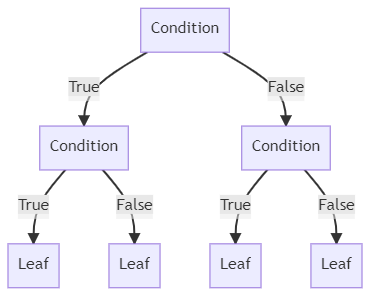
\includegraphics[width=0.5\linewidth]{images/DecisionTree.png}
    \caption{Example of decision tree model}
    \label{fig:dt}
\end{figure}

\newpage

\section{Differentiable Decision Tree}
\label{sec:160}
In order to apply a policy gradient method such as PPO, which cannot work with discrete DTs because of was designed for neural networks, DTs require some modification to get the so-called Differentiable Decision Trees (DDTs).

The approach proposed first in \cite{suarez} and thereafter taken and used by A. Silva et al. in \cite{silva} is to replace the Boolean condition in the decision nodes with a sigmoid activation function.

This method has also been used for this work.
\newpage

      \emptypage
      \chapter{Setup main algorithm and models}
\label{cha:200}
The concept of this work is to evolve DTs using an evolutionary algorithm, in this case Grammatical Evolution, and then, every \textit{n} number of generations, the best or a random tree is chosen from the population with a probability of 50\(\%\) each: in this way I give the same probability to \textit{exploit}, choosing the best tree, and to \textit{explore}, choosing a random tree. Thus the selected tree is converted into a DDT and sent to the PPO algorithm, which seeks to optimize it leaving the structure unchanged. When this optimization part finishes, the DDT is discretized back into a DT and then the new fitness of the individual is calculated on 50 different episodes in the environment. Lastly, the best individual is selected also considering this new optimized policy from PPO and the evolutionary process going on with the next generations.


\section{Setup for GE}
\label{sec:210}
To evolve individuals during most generations, it has been used Grammatical Evolution. The first generation is composed by random individuals created by a factory which takes directives on how to create them from a \textit{yaml} configuration file. In the configuration file in fact are present some data necessary to initiate GE, listed below:
\begin{itemize}
    \item \textit{geno\_len}, which is the maximum length of the genotype strings that make up the individuals
    \item \textit{pop\_size}, which indicates how many individuals are in the population
    \item \textit{tournament\_size}, which states for the dimension of the tournament selection operator; tournament selection works as follow: for every offspring to be generated, \textit{k} (\textit{k} is the tournament size) random individuals are picked from the population, then the individual with the highest fitness is chosen and a copy is made
    \item \textit{gene\_prob}, which is a float number that specifies with what probability a particular gene can mutate applying mutation operator
    \item \textit{grammar}, which is the most important parameter because with this is created all the individuals respecting the defined constraints (e.g. the dimension of the input state space and the boundaries for values in the condition splits).
    
    The grammar is expressed in the form of production rules using the Backus-Naur From (BNF) notation. BNF grammars consist of \textit{terminals}, which are items that can appear in the language, e.g., $+$, $-$, etc., and \textit{nonterminals}, which can be expanded into one or more terminals an nonterminals. A grammar can be represented by the tuple $\{N,T,P,S\}$, where $N$ is the set of nonterminals, $T$ the set of terminals, $P$ a set of production rules that maps the elements of $N$ to $T$, and $S$ is a start symbol that is a member of $N$ \cite{neill}.
    \item \textit{generations}, which is the number of iterations for the EA
\end{itemize}
Afterward the evolutionary process starts and the mutations and crossovers are made depending on a probability value, which for this work were 100\(\%\) and 0\(\%\) respectively. The reason why the crossover probability is set to 0 is because in GE the crossover operator may have destructive impact on the process.

When the new population of changed individuals is obtained, the fitness function values it in order to assign the fitness to every individual.

Then, the replacement takes place, substituting the individuals of the new population (i.e. the offspring) with the individuals of the old population (i.e. the parents) if their fitness is better. This process is repeated for \textit{generations} times where the individuals changed even drastically in the structure and in the features chosen for the splits.

At regular intervals, also PPO is applied to the population. The main idea is that GE helps individuals select the best features for splits and put them in the correct order in the structure of the tree, while PPO works on \textit{split\_values} in the condition nodes and on \textit{actions} in the leaves, trying to maximize the reward in the environment.


\section{Converting DTs in DDTs and vice versa}
\label{sec:220}
As it was explained in the introduction chapter, PPO cannot be applied to discrete DTs.

First of all, is necessary to convert them into DDTs and for this purpose I followed the method used in \cite{silva}: the Boolean conditions of DTs, shown in Eq. 1, in which \textit{x} and \(\phi\) stand for the selected feature and the split value respectively, are substituted with a sigmoid activation function, shown in Eq. 2, where \(\alpha\) is a steepness parameter which helps to give more weight to one branch rather then the other, making the split less "\textit{soft}", and \(\phi\) is, as before, the split value.
\[\mu(x) :=
\begin{cases}
1,\quad if $\>$ \textit{x} < \phi\\
0,\quad o/w
\end{cases}
\quad(1)
\]
\[\mu(x) := \frac{1}{1+e^{-\alpha(x-\phi)}}\qquad\quad(2)\]
Furthermore, the constant leaves in DTs, which simply contain an integer indicating the mapped action in the environment, are replaced with differentiable leaves, composed of a tensor of dimension equal to the action space dimension and where in each position there is the probability of taking the action mapped with that particular index (e.g. looking at a leaf like this: [0.3, 0.7], it means that there is 30\(\%\) of taking the action 0 and 70\(\%\) of taking the action 1).

The conversion from constant leaf to differentiable leaf works as follow: the action that was previously saved in the constant leaf and the action space dimension are passed as parameters in the \textit{init} function; then a tensor filled with 0.0 is created and exclusively the value in the position corresponding to the passed action is substituted and augmented using the method exposed in the Eq. 3, to give more percentage of choosing that particular action in PPO, leading to greater stability of the algorithm. After this process, the real tensor of probabilities is created through a Gaussian distribution, using the previous tensor as mean and with \(\sigma\) equal to 0.1. Finally, a \textit{Softmax} is applied to the tensor to re-scale the elements so that lie in the range [0,1] and sum to 1.

Both in condition nodes and in leaves it's important to specify the \textit{requires\_grad()} PyTorch function in order to track of operations on tensors with the aim of making backpropagation possible during PPO.
\[tensor[action] = n\_action-1\qquad\quad(3)\]
The reverse method is done simply by recreating orthogonal conditions using \textit{input\_features} and \textit{split\_values} from differentiable conditions for the condition nodes and initializing constant leaves with action chosen using an \textit{argmax} on the probability tensor from differentiable leaves for the leaves.


\section{Forward method in DDTs}
\label{sec:230}
The forward method in DDTs works differently in comparison with the method for DTs, where simply it's necessary to evaluate the Boolean condition for every condition node at each state, choose the correct path and then return the action contained in a leaf.

In a DDT, when the state tensor containing the observation data collected from the environment is given to the tree, every branch of the tree is taken because of the sigmoid activation function, which also determines the weight assigned to every specific branch, and the forward method thus return a weighted averages of the probability tensors in the leaves. For not making that splits \textit{"fuzzy"}, the \(\alpha\) parameter shown in Eq. 2 is set to 1000, a value found heuristically which guarantees that the weights earned by sigmoid activation function are equal to 0 or 1: this way it's as if we just take the correct path by having a discrete DT and the backpropagation only changes the conditions and the leaf that were really needed to determine the output label given an input state. An \(\alpha\) parameter set with a lower value doesn't give the security to have a discrete split with 0/1 weight.


\section{Pruning method for DTs}
\label{sec:240}
To prune the individuals obtained during the evolutionary process in order to make them even more interpretable, it was used a simplification mechanism taken from \cite{custode}.

First, the policy (e.g. the individual) is executed in a validation environment for 100 episodes, to be sure to try every possible case. Every time a node is visited during this process, a counter (each node has one) is increased. Once this phases is finished, every node that have the counter equal to 0 (those that have not been visited) is removed. Lastly, there's an iteratively search for nodes whose action in the left leaf equals the one in the right leaf: each time a node like this is found, it is replaced with a leaf that contains the action in common to the two leaves. The process finishes when the tree does not contain nodes of this type.

This last mechanism is very useful as PPO often produces trees where nodes have the same actions in the leaves (because it switches actions in leaves).

The simplification process is feasible even by hand in a short time, since the task and the environment are not too complex. For more details on this, see the dedicated Section \ref{sec:prune} in the supplementary material.


\section{Metric for interpretability}
\label{sec:250}
To measure the complexity of the policies, from the point of view of interpretability, I used the metric first proposed in \cite{metric} and then revised in \cite{custode}, shown in Eq.4.
\[\mathcal{M}=-0.2+0.2l+0.5n_o+3.4n_{nao}+4.5n_{naoc}\qquad\quad(4)\]
The parameters that appear in the formula are:
\begin{itemize}
    \item $l$, sum of operations, variables and constants
    \item $n_o$, the number of operations
    \item $n_{nao}$, the number of non-arithmetical operations
    \item $n_{naoc}$, the number of consecutive compositions of non-arithmetical operations
\end{itemize}
This metric is interpreted as follows: a higher $\mathcal{M}$ for a model means that that model is harder to interpret (e.g. a DT composed only by a constant, which is the best case from the interpretability point of view, has complexity equal to 0).
\newpage
      \emptypage
      \chapter{Setup PPO and link it with GE}
\label{cha:300}
Once the DTs are converted into DDTs, they are ready to be optimized via PPO, but before it's necessary to modify the existing algorithm to accept them. The code for an implementation of basic PPO has been taken from \cite{barhate} written with PyTorch library, in which I did all the modifications needed for the purpose, explained in the next section.
 
 
\section{Modifying PPO to accept DDTs}
\label{sec:310}
PPO is a policy gradient method that trains a stochastic policy in an on-policy way. Also, it utilizes the Actor Critic method. So PPO works with 2 Neural Networks (NNs), one as the actor, which chooses the action given a state, and the other as the critic, which evaluates the expected reward given a state. The main thing to do was to replace the actor with the DDT passed to the optimizer and then change the forward method of the first NN to the forward method explained in the Section \ref{sec:230}. The critic instead remaining a NN as before.\\
Next, other modifications was suggested in \cite{silva} and listed below:
\begin{itemize}
    \item the optimizer used is RMSprop and the parameters taken are the ones from the critic and the ones from the DDT, which are the split values and the probability tensors of the leaves;
    \item the activation function for the critic (a NN) is ReLU().
\end{itemize}



\section{Tuning the hyperparameters}
\label{sec:320}
All the PPO's hyperparameters used were found by a manual tuning, trying to find the best values for each environment. Being several parameters, it would have been difficult to obtain the ones that gain the optimum results for every environment, so for this work I settled on parameters that gave me the security to improve the DDT even if sometimes the algorithm doesn't work as expected.

For this reason the algorithm in general would require a more in-depth study, looking for the best configuration settings with the help of a tool that would reduce the effort to find them, trying a large scale of configurations autonomously.

For the PPO's hyperparameters and also the parameters to configure the environment, see the supplementary material in the appendix.

\section{Connecting PPO with GE}
\label{sec:330}
Once the algorithm was ready to be used, I implemented a method that chooses every \textit{n} generations, where \textit{n} varies depending on the environment considered, the best tree or a random tree with $50\%$ probability each.

Some checks to the DTs that need to be chosen were added in order to not waste time trying to optimize a tree that cannot be improved. The checks that I have carried out are the following:
\begin{itemize}
    \item Check if the chosen DT already solves the task (see the Chapter \ref{cha:400} for the thresholds for every environment).
    \item Check if the DT is composed only by 1 leaf, because it's impossible to optimize it.
    \item Check if the DT has only 1 condition and 2 leaves, because even in the simplest environment (i.e. CartPole-v1) a DT with these characteristics is not able to solve the task.
\end{itemize}

When at least one of the conditions listed above is met, then another random DT is chosen from the population. There's another final check on the times this procedure can happen and it's equal to the \textit{population size}: in the case that all the individuals in the population solve the task or have a structure that does not allow them to solve it, PPO cannot do anything to improve the evolutionary process and it's necessary to wait for the next generations.

After choosing the DT to be improved, it's converted into a DDT using the technique explained in Chapter \ref{cha:200}, Section \ref{sec:220} and sent to PPO.

When the DDT is returned to the main algorithm, first of all it's discretized back into a DT.

At this point of the implementation, a problem concerning the method to put back the individual into the population came up and it could be solved in two ways.

The first idea was to replace the individual directly in the population, substituting  the worst one; but this would have required a particular function which makes possible the conversion from phenotype to genotype, because the optimization with PPO is done directly on the phenotype of the individuals. This mapping process is really tricky to do, despite the conversion from genotype to phenotype is quite easy (it's the basis for GE), so it was thought to bypass the problem by not putting the individual back in the population. This leads to an obvious consequence: that of not really improving the evolutionary process.

So I decided to focus more on the optimization of the DTs with PPO, comparing them with the un-optimized version, because it might be possible that some particular individuals with a specific genotype that have a low fitness could be transformed into an high-score individuals by small changes directly on the phenotype (using PPO).

Additionally to what I said above, even if the individual optimized is not put back into the population, it's compared with the best DT of the current generation to see if a new best was found thanks to PPO.

\newpage
      \chapter{Testing}
\label{cha:400}
In the following sections there are all the cases considered, with a brief definition of the tasks, and are present the configuration settings used for each specific environment. Finally the results of the tests were reported for each case and there are some consideration deduced from them, with the last section containing the interpretability study, which is a key aspect in IAI.

What I expected is that PPO would be able to optimize a lot of the individuals given to it, even if they wouldn't be able to solve completely the task, because the orthogonal DTs with constant leaves used are often too simple to solve the more complex environments. Despite this premise, I expected that sometimes, for the simplest environment (i.e. CartPole-v1) PPO would produce a DT with a maximum fitness, solving the task.

For this work, it were considered three environments, two have a sparse reward and the other one not, to see how PPO behaves in these two different situations.

\textit{Note:} all the environments considered has a discrete action space.


\section{CartPole-v1}
\label{sec:410}
\subsection{Definition}
\label{subsec:411}
A pole is attached by an un-actuated joint to a cart, which moves along a frictionless track. The pendulum is placed upright on the cart and the goal is to balance the pole by applying forces in the left and right direction on the cart \cite{gym} \cite{cartpole}.\\[0.3in]
The \textit{\textbf{state}} of the environment has dimension equals to 4 and is composed of:
\begin{itemize}
    \item Cart position: \textit{x} \(\in\) [-4.8, 4.8] m
    \item Cart velocity: \textit{v} \(\in\) ]-\(\infty\), \(\infty\)[ m/s
    \item Pole angle: \textit{\(\theta\)} \(\in\) [-0.418, 0.418] rad
    \item Pole angular velocity: \textit{\(\omega\)} \(\in\) ]-\(\infty\), \(\infty\)[ rad/s
\end{itemize}
The \textit{\textbf{actions}} that the agent can perform are:
\begin{itemize}
    \item Move left (applying a 10N force to the cart)
    \item Move right (applying a 10N force to the cart)
\end{itemize}
The agent receives a \textit{\textbf{reward}} of +1 for every step taken.\\[0.1in]
The \textit{\textbf{termination criterion}} is one of the following:
\begin{itemize}
    \item Pole angle \textit{$\theta$} is greater than $\pm$ 0.2095 rad
    \item Cart position \textit{x} is greater than $\pm$ 2.4 (center of the cart reaches the edge of the display)
    \item Episode length is greater than 500
\end{itemize}
The task is considered \textit{\textbf{solved}} if the agent obtains a mean reward \textit{R} \(\geq\) 475 on 100 runs.


\subsection{Settings}
\label{subsec:412}
The grammar used is shown in the Table \ref{table:1}. The settings used for GE is shown in the Table \ref{table:2}. The parameters are taken from \cite{custode} and was made a modification for some of them by a manual tuning.
\newpage


\captionsetup{margin=2cm}
\begin{table}[h!]
\begin{center}
\begin{tabular}{ |c|c| }
\hline
\textbf{Rule} & \textbf{Production} \\
\hline
dt & \textit{$< if >$}\\
if & \textit{$if < condition > then < action > else < action >$}\\
condition & \textit{lt$(input\_feature,<constant>)$}\\
action & \textit{leaf $| < if >$}\\
constant & $[-4.8, 4.8]$ with step 0.005\\
\hline
\end{tabular}
\caption{Grammar used to evolve orthogonal decision trees in the CartPole-v1 environment. The symbol "$|$" indicates that there is the possibility to choose between different symbols. Input\_feature stands for one of the possible inputs taken from the state space.}
\label{table:1}
\end{center}
\end{table}


\begin{table}[h!]
\begin{center}
\begin{tabular}{ |c|c| } 
\hline
\textbf{Parameter} & \textbf{Value} \\
\hline
Population size & 200\\
Generations & 200\\
Genotype length & 100\\
Crossover probability & 0\\
Mutation probability & 1\\
Mutation type & Uniform, with gene probability = 0.1\\
PPO & every 40 generations\\
\hline
\end{tabular}
\caption{Parameters used for the Grammatical Evolution with orthogonal decision trees in the CartPole-v1 environment.}
\label{table:2}
\end{center}
\end{table}


\subsection{Results}
\label{subsec:413}
The results are shown in the Table \ref{table:scoreCP}. For the considerations made in chapter \ref{cha:300}, they take into account not only the fitness of individuals optimized with GE, but also the ones from PPO.

The task was solved by the agent 9 times on 10 runs ($90\%$ of the cases), with only a low fitness on Run2. In particular PPO was applied every 40 generations, so 4 times per run for a total of 40 PPO runs during all the training processes. Of these 40, in 29 runs PPO brought an improvement of the fitness of the individuals and in 4 of these 29 runs it has generated a maximum score in the generations in which it was applied.

To better see the optimization that PPO has done to individuals, in Figure \ref{fig:ComparisonSingleCP} are shown in particular 3 runs of the 10 runs made in which PPO greatly affects the convergence towards the solved threshold. In this figure is possible to notice, looking for example the fitness for the best individual of Run4, that it reached the state-of-the-art reward during the 40th generation, thanks to PPO; comparing it with the same test, without using PPO, it reached the state of the art only during the 128th generation, so 88 generations later. In this case, PPO was able to save the $68.75\%$ of generations, which is a huge improvement. Similar cases are Run1 and Run3.

In Figure \ref{fig:BestTreeCP} is shown the best DT obtained from PPO for the Run4, during the 40th generation (the case discussed before): before applying PPO, it had a fitness of 9.4 and after the algorithm has been applied, it obtains a score of 499.8, averaged on 100 unseen episodes in the environment, solving the task. This demonstrates that sometimes a particular genotype contains the potential to gain an high score, having good \textit{input\_features} in the decision nodes and need only small changes on \textit{split\_values} or in constant leaves: in fact PPO, in this case, changed some actions contained in the leaves (from \textit{move\_left} to \textit{move\_right} or vice versa) and this led to an enormous improvement in terms of fitness because it upended completely the behaviour of the individual.

Finally in the Figure \ref{fig:CartPoleMean} is shown the training mean best fitness for each generation averaged across all the 10 runs. The orthogonal decision trees are able to converge to the fitness threshold which indicates that the task is solved.

Differently from results in \cite{custode}, here the algorithm takes more generations to converge and also in a case it wasn't able to create in time a policy to solve the task: mainly this is due to the fact that I used constant leaves for this work, while in that paper were used \textit{QLearningLeaves}, so the leaves were able to learn the best action using the Q Learning algorithm.

Concluding, with the promising results obtained via PPO shown above, I can say that if it had been possible to put back into the population all the optimized individuals from PPO, using them to do crossover or mutation, the whole evolutionary algorithm would have benefited from it, reducing the number of generations needed to converge towards this threshold.

To see the complete version of the DT in Figure \ref{fig:BestTreeCP} and how it was pruned, look at the supplementary material.
\vspace{0.3in}

\begin{table}[h!]
\begin{center}
\begin{tabular}{ |c|c|c|c|c| } 
\hline
\textbf{Run} & \textbf{Seed} & \textbf{Training Best Fitness} & \textbf{Testing Best Fitness} & $\mathcal{M}$\\
\hline
R1 & 0 & \textbf{500.00} & \textbf{500.00} & 53.4\\
R2 & 1 & 234.8 & 199.71 & 35.6\\
R3 & 2 & \textbf{500.00} & \textbf{487.40} & 53.4\\
R4 & 3 & \textbf{500.00} & \textbf{499.28} & 53.4\\
R5 & 4 & \textbf{500.00} & \textbf{488.20} & 35.6\\
R6 & 5 & \textbf{500.00} & \textbf{498.05} & 53.4\\
R7 & 6 & \textbf{500.00} & \textbf{486.26} & 53.4\\
R8 & 7 & \textbf{500.00} & \textbf{500.00} & 35.6\\
R9 & 8 & \textbf{500.00} & \textbf{493.96} & 53.4\\
R10 & 9 & \textbf{500.00} & \textbf{498.8} & 53.4\\
\hline
\end{tabular}
\caption{Reward obtained by the best policy with orthogonal decision trees on CartPole-v1 environment (bold denotes the solved ones)}
\label{table:scoreCP}
\end{center}
\end{table}

\begin{figure}[h!]
    \centering
    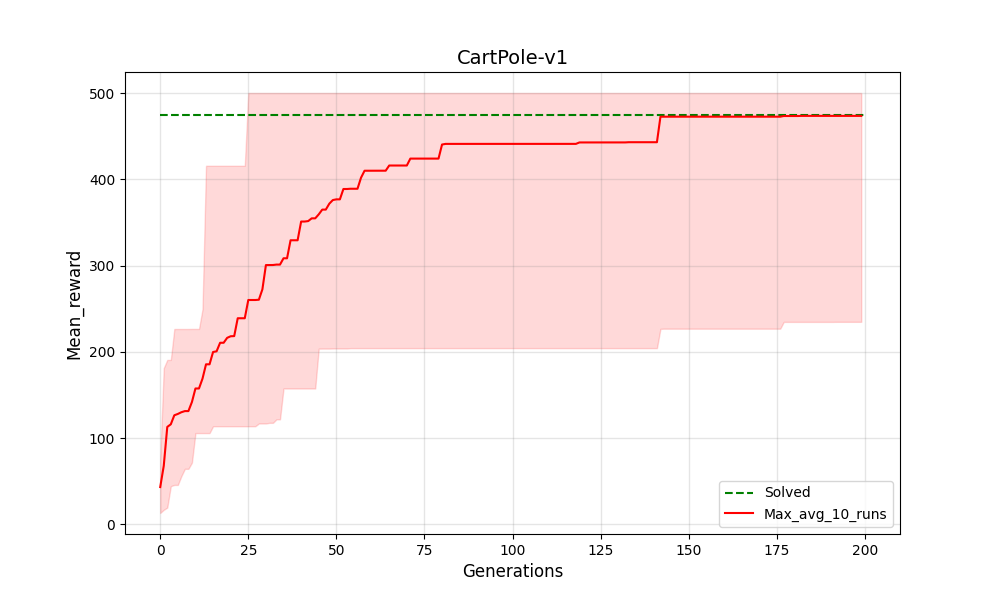
\includegraphics[width=1\linewidth]{images/CartPole/CartPole10run.png}
    \caption{Total training mean reward with orthogonal decision trees in the CartPole-v1 environment, using both GE and PPO}
    \label{fig:CartPoleMean}
\end{figure}

\newpage

\begin{figure}[h!]
    \centering
    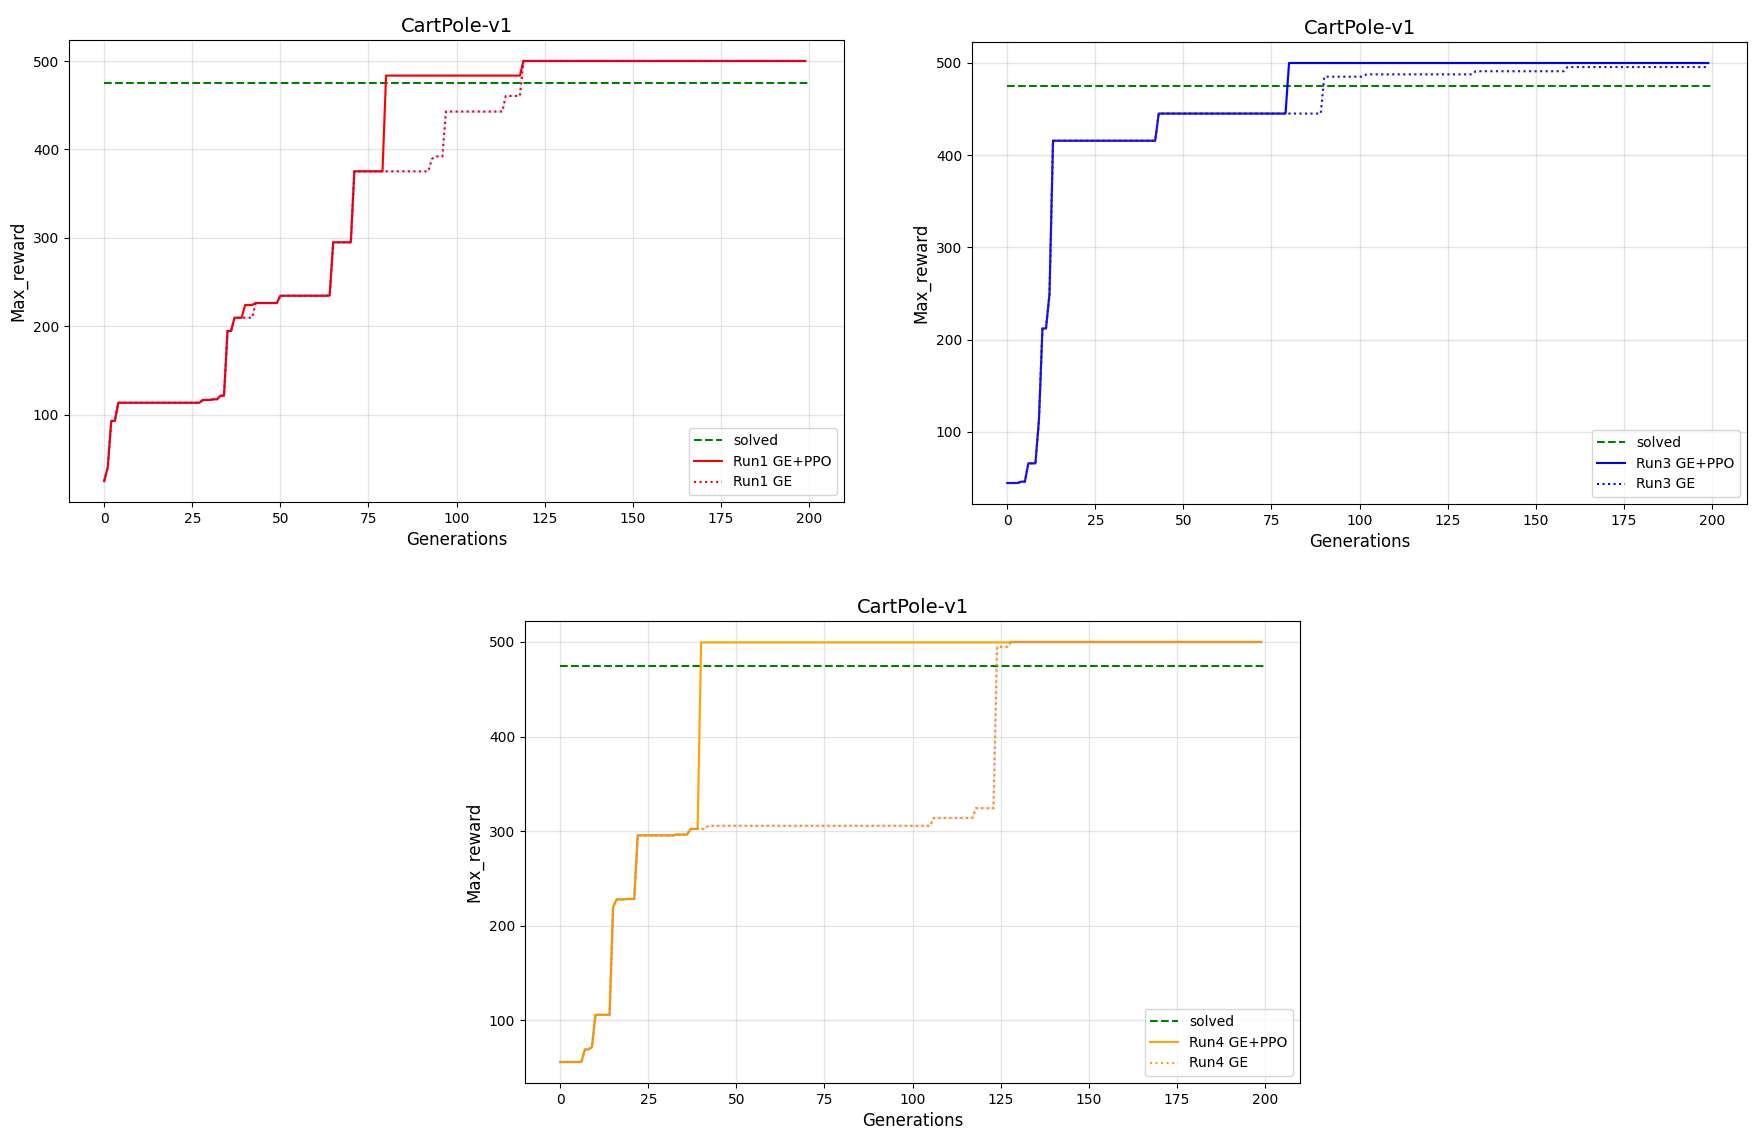
\includegraphics[width=1\linewidth]{images/CartPole/mixedRunSingle.png}
    \caption{Comparison between fitnesses for Run1, Run3 and Run4. The solid line represents the results using both GE and PPO, instead the dotted line represents the results considering only GE}
    \label{fig:ComparisonSingleCP}
\end{figure}

\begin{figure}[h!]
    \centering
    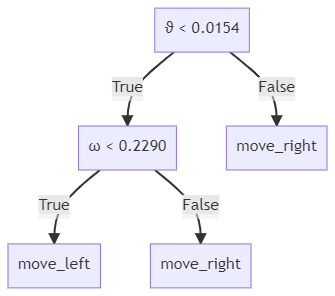
\includegraphics[width=0.4\linewidth]{images/CartPole/bestPPOprunedCP.png}
    \caption{The best tree optimized by PPO in CartPole-v1 environment, pruned by eliminating unnecessary branches}
    \label{fig:BestTreeCP}
\end{figure}

\newpage



\section{Acrobot-v1}
\label{sec:420}
\subsection{Definition}
\label{subsec:421}
The system consists of two links connected linearly to form a chain, with one end of the chain fixed. The joint between the two links is actuated. The goal is to apply torques on the actuated joint to swing the free end of the linear chain above a given height while starting from the initial state of hanging downwards \cite{gym} \cite{acrobot} \cite{sutton}.\\[0.3in]
The \textit{\textbf{state}} of the environment has dimension equals to 6 and is composed of:
\begin{itemize}
    \item Cosine of \(\theta_1\): \textit{cos(\(\theta_1\))} \(\in\) [-1, 1]
    \item Sine of \(\theta_1\): \textit{\(sin(\theta_1\))} \(\in\) [-1, 1]
    \item Cosine of \(\theta_2\): \textit{cos(\(\theta_2\))} \(\in\) [-1, 1]
    \item Sine of \(\theta_2\): \textit{sin(\(\theta_2\))} \(\in\) [-1, 1]
    \item Angular velocity of \(\theta_1\): \textit{\(\omega_1\)} \(\in\) [-4\(\cdot\pi\), 4\(\cdot\pi\)] rad/s
    \item Angular velocity of \(\theta_2\): \textit{\(\omega_2\)} \(\in\) [-9\(\cdot\pi\), 9\(\cdot\pi\)] rad/s
\end{itemize}
The \textit{\textbf{actions}} that the agent can perform are:
\begin{itemize}
    \item Apply -1 torque to the actuated joint
    \item Apply 0 torque to the actuated joint
    \item Apply 1 torque to the actuated joint
\end{itemize}
The agent receives a \textit{\textbf{reward}} of -1 for each timestep. When it reaches the target height, it receives a reward equals to 0.\\[0.1in]
The \textit{\textbf{termination criterion}} is one of the following:
\begin{itemize}
    \item The free end reaches the target height, which is constructed as: \(-\cos(\theta_1) - \cos(\theta_2 + \theta_1) > 1.0\)
    \item Episode length is greater than 500
\end{itemize}
The task is considered \textit{\textbf{solved}} if the agent obtains a mean reward \textit{R} \(\geq\) -100 on 100 runs.


\subsection{Settings}
\label{subsec:422}
The grammar used is shown in the Table \ref{table:5}. The settings used for GE is shown in the Table \ref{table:6}. The parameters were found by a manual tuning.


\captionsetup{margin=2cm}
\begin{table}[h!]
\begin{center}
\begin{tabular}{ |c|c| }
\hline
\textbf{Rule} & \textbf{Production} \\
\hline
dt & \textit{$< if >$}\\
if & \textit{$if < condition > then < action > else < action >$}\\
condition & \textit{lt$(input\_feature,<constant>)$}\\
action & \textit{leaf $| < if >$}\\
constant & $[-28.27, 28.27]$ with step 0.001\\
\hline
\end{tabular}
\caption{Grammar used to evolve orthogonal decision trees in the Acrobot-v1 environment. The symbol "$|$" indicates that there is the possibility to choose between different symbols. Input\_feature stands for one of the possible inputs taken from the state space.}
\label{table:5}
\end{center}
\end{table}


\begin{table}[h!]
\begin{center}
\begin{tabular}{ |c|c| } 
\hline
\textbf{Parameter} & \textbf{Value} \\
\hline
Population size & 200\\
Generations & 50\\
Genotype length & 100\\
Crossover probability & 0\\
Mutation probability & 1\\
Mutation type & Uniform, with gene probability = 0.1\\
PPO & every 15 generations\\
\hline
\end{tabular}
\caption{Parameters used for the Grammatical Evolution with orthogonal decision trees in the Acrobot-v1 environment.}
\label{table:6}
\end{center}
\end{table}


\subsection{Results}
\label{subsec:423}
The results are shown in the Table \ref{table:scoreAB}. The task was solved by the agent in $100\%$ of the cases, during 10 runs. This result doesn't surprise me, being Acrobot-v1 an environment little more complex than CartPole-v1 environment (because it has an higher input and action dimension), but still an easy one.

PPO was applied every 15 generations, so 3 times per run for a total of 30 PPO runs during all the training processes. During this 30 runs, in the majority of the cases PPO was not able to improve the individuals (lowering the fitness of the individual or maintaining the previous one), with only a few weak optimizations, resulting in a non efficient process.

In addition, PPO has never obtained an individual that has the best fitness for the generation in progress, so it didn't accelerate really the process to converge the maximum fitness to the optimal one. This last statement is obvious also because I applied PPO starting from the 15th generation onward and, looking the plot of the fitnesses in Figure \ref{fig:AcrobotMean}, it's possible to notice that the average max during all the runs has passed the solved threshold very quickly, around the 8th-9th generation.

Despite this, PPO could also have found a new maximum for the evolutionary process (as it happened for CartPole-v1), but unfortunately was not this the case.

In total, PPO never improved an individual by getting it to solve the task; I reported the best one optimized via PPO in Figure \ref{fig:BestTreeAB}, in a pruned version, even if its average reward during the testing phase in the environment is lower than the -100.0 solved threshold (it obtains a reward equals to -113.89, averaged on 100 unseen episodes). Looking at each single score in the environment, I discovered that in 36 of this 100 testing runs, the model was able to solve the task, also obtaining sometimes the maximum reward of -81.0; on the other hand, it also obtained sometimes -245.0, which greatly lowers the total mean; this denotes that the policy is not steady enough, leading to solve the task only occasionally.

The original policy was deeper and more complex and is visible in the Figure \ref{fig:TreeFullAB} in the appendix, but many branches were impossible to take, so they have been pruned off, obtaining a tree with depth equals to 3 (for the full simplification process, see the dedicated appendix section).

Talking about the motivation for which the results from PPO are so negative, this is due to the fact that the Acrobot-v1 environment, as MountainCar-v0, has a sparse reward: this means that the reward is obtained from the environment only if it can reach the termination criterion (for this environment is that the free end reaches a target height), differently from CartPole-v1. Being PPO an on-policy algorithm, it means that it collects data from a certain amount of episodes and after it performs a policy gradient update. Reaching the target height with random actions (obtained from a random policy) or a non perfectly optimized policy (the ones that are sent to PPO) is a really rare event and when it happens, it's unlikely that a single positive reward affects the process so much. This leads PPO to get stuck for the majority of the times during the entire optimization process and explains the bad results overall.

This statement was confirmed in \cite{ppo_acrobot}, where the author was not able to solve the Acrobot-v1 task with PPO, and the reason was corroborated in \cite{ppo_mountaincar}.

For this reason it was also added a constraint, in addition to those present in the Section \ref{sec:330}, to the individuals that could be optimized via PPO, to improve the process; the additional constraint is that the random individual to be chosen cannot have a fitness equals to -500.0 (the lowest for the Acrobot-v1 environment). In this way I helped a bit the optimization process, being sometimes useful to improve, even a bit, some individuals.

In conclusion, it was not worth applying PPO in this environment due to the sparse reward and the algorithm didn't help the fitness to reach the solved threshold, although the task is one of the easiest in the \textit{Classic Control} library.
\vspace{0.3in}

\begin{table}[h!]
\begin{center}
\begin{tabular}{ |c|c|c|c|c| } 
\hline
\textbf{Run} & \textbf{Seed} & \textbf{Training Best Fitness} & \textbf{Testing Best Fitness} & $\mathcal{M}$\\
\hline
R1 & 0 & \textbf{-81.0} & \textbf{-83.43} & 35.6\\
R2 & 1 & \textbf{-80.0} & \textbf{-88.71} & 35.6\\
R3 & 2 & \textbf{-81.2} & \textbf{-88.07} & 35.6\\
R4 & 3 & \textbf{-75.4} & \textbf{-84.85} & 71.2\\
R5 & 4 & \textbf{-76.4} & \textbf{-82.32} & 35.6\\
R6 & 5 & \textbf{-83.6} & \textbf{-84.23} & 17.8\\
R7 & 6 & \textbf{-74.2} & \textbf{-83.94} & 35.6\\
R8 & 7 & \textbf{-70.4} & \textbf{-87.91} & 35.6\\
R9 & 8 & \textbf{-83.0} & \textbf{-83.87} & 35.6\\
R10 & 9 & \textbf{-87.6} & \textbf{-85.03} & 53.4\\
\hline
\end{tabular}
\caption{Reward obtained by the best policy with orthogonal decision trees on Acrobot-v1 environment (bold denotes the solved ones)}
\label{table:scoreAB}
\end{center}
\end{table}


\begin{figure}[h!]
    \centering
    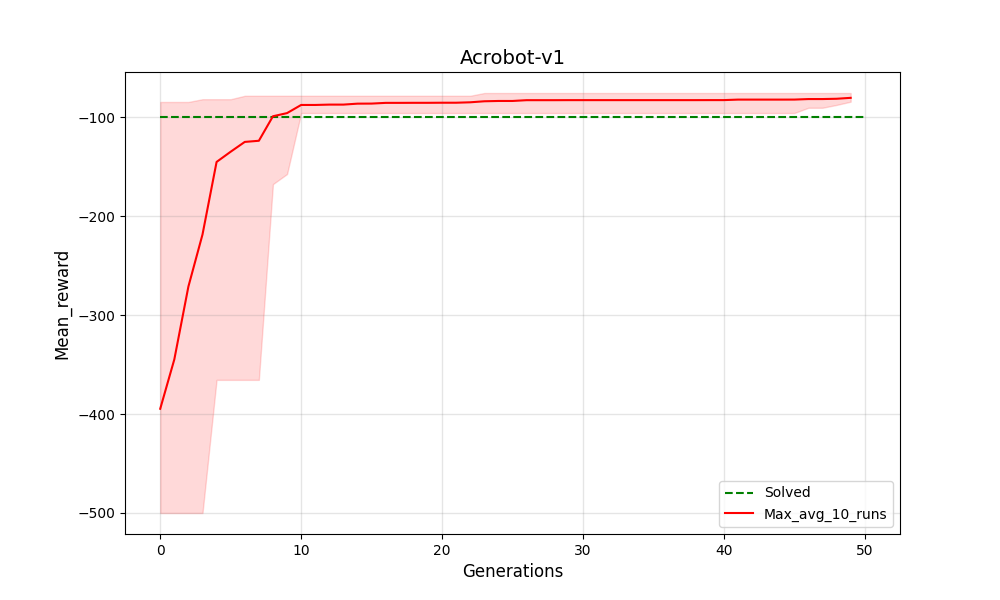
\includegraphics[width=1\linewidth]{images/Acrobot/Acrobot10run.png}
    \caption{Total training mean reward with orthogonal decision trees in the Acrobot-v1 environment, using both GE and PPO}
    \label{fig:AcrobotMean}
\end{figure}

\begin{figure}[h!]
    \centering
    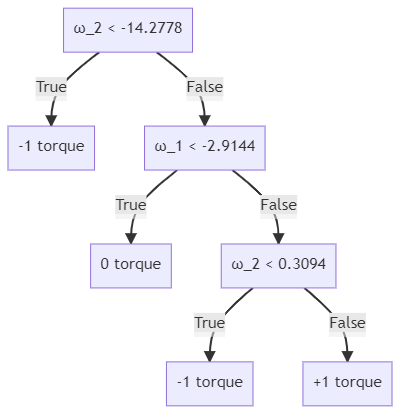
\includegraphics[width=0.4\linewidth]{images/Acrobot/bestPPOprunedAB.png}
    \caption{The best tree optimized by PPO in Acrobot-v1 environment, pruned by eliminating unnecessary branches}
    \label{fig:BestTreeAB}
\end{figure}

\newpage

\section{MountainCar-v0}
\label{sec:430}
\subsection{Definition}
\label{subsec:431}
The Mountain Car MDP is a deterministic MDP that consists of a car placed stochastically at the bottom of a sinusoidal valley, with the only possible actions being the accelerations that can be applied to the car in either direction. The goal of the MDP is to strategically accelerate the car to reach the goal state on top of the right hill \cite{gym} \cite{mountaincar}.\\[0.3in]
The \textit{\textbf{state}} of the environment has dimension equals to 2 and is composed of:
\begin{itemize}
    \item Position of the car along the x-axis: \textit{x} \(\in\) [-1.2, 0.6] m
    \item Velocity of the car: \textit{v} \(\in\) [-0.07, 0.07] m/s
\end{itemize}
The \textit{\textbf{actions}} that the agent can perform are:
\begin{itemize}
    \item Accelerate to the left
    \item Don't accelerate
    \item Accelerate to the right
\end{itemize}
The agent is penalised receiving a \textit{\textbf{reward}} of -1 for each timestep.\\[0.1in]
The \textit{\textbf{termination criterion}} is one of the following:
\begin{itemize}
    \item Episode length is greater than 200 timesteps
    \item The position of the car is greater than or equal to 0.5 (the goal horizontal position on top of the right hill)
\end{itemize}
The task is considered \textit{\textbf{solved}} if the agent obtains a mean reward \textit{R} \(\geq\) -110 on 100 runs.


\subsection{Settings}
\label{subsec:432}
The grammar used is shown in the Table \ref{table:3}. The settings used for GE is shown in the Table \ref{table:4}. The parameters are taken from \cite{custode} and was made a modification for some of them by a manual tuning.


\captionsetup{margin=1.7cm}
\begin{table}[h!]
\begin{center}
\begin{tabular}{ |c|c| }
\hline
\textbf{Rule} & \textbf{Production} \\
\hline
dt & \textit{$< if >$}\\
if & \textit{$if < condition > then < action > else < action >$}\\
condition & \textit{lt$(input\_feature,<constant>)$}\\
action & \textit{leaf $| < if >$}\\
constant & $[-1.2, 0.6]$ with step 0.005\\
\hline
\end{tabular}
\caption{Grammar used to evolve orthogonal decision trees in the MountainCar-v0 environment. The symbol "$|$" indicates that there is the possibility to choose between different symbols. Input\_feature stands for one of the possible inputs taken from the state space.}
\label{table:3}
\end{center}
\end{table}


\begin{table}[h!]
\begin{center}
\begin{tabular}{ |c|c| } 
\hline
\textbf{Parameter} & \textbf{Value} \\
\hline
Population size & 200\\
Generations & 1000\\
Genotype length & 1024\\
Crossover probability & 0\\
Mutation probability & 1\\
Mutation type & Uniform, with gene probability = 0.05\\
PPO & in the 50th-100th-400th-800th generation\\
\hline
\end{tabular}
\caption{Parameters used for the Grammatical Evolution with orthogonal decision trees in the MountainCar-v0 environment.}
\label{table:4}
\end{center}
\end{table}

\subsection{Results}
\label{subsec:433}
The results are shown in the Table \ref{table:scoreMC}. As for all the others environment, also here the results take in account the optimized individuals from PPO.

In this case, the task was much more difficult than the previous ones: for this reason, it was needed to increase not only the number of generations of the process, but also the maximum genotype length to be able to obtain more complex DTs. Those modifications are shown in the configuration settings for GE in the Table \ref{table:4}. A consequence of raising those parameters is obviously that the evolutionary process takes more time to be carried out; moreover, increasing the maximum genotype length slows down the "decision" process, because the trees generated from the algorithm could have very high depth and it takes more time to visit all the nodes that are needed to take the decision (remember that during PPO optimization all the nodes are visited for each decision that has to be taken).

\textit{Note:} also in this experiment I added the same constraint as the one added in Acrobot-v1 environment (that the individuals with the minimum fitness cannot be optimized by PPO) because also MountainCar has a sparse reward and for this reason PPO does not work well being an on-policy algorithm, as explained by \cite{ppo_mountaincar}. This additional condition helps a bit the optimization process, not wasting time on that type of individuals.

The task was solved in the $50\%$ of the cases, during 10 runs (in all the runs where it wasn't able to solve the task, the optimization has stalled with a policy that obtains a reward very close to the solved threshold).

In total, PPO was applied 4 times every run, for a total of 40 PPO runs (39 to be precise, because, during the 50th generation on the 6th run, no individuals of the populations met all the constraint defined in the Section \ref{sec:330}).

For this experiment, I decided not to apply PPO every \textit{"n"} generations but I choose to put the optimization process via PPO in specific points (4 in all, in line with the other tests), during the 50th, the 100th, the 400th and the 800th generation. I chose those particular generations because I wanted to optimize the population during different phases of the evolutionary process: the first two seek to speed up the convergence towards the solved threshold; the other two placed at the 400th and at the 800th generation, when the algorithm has probably already solved the task, try to improve the final result (getting the state-of-the-art) or possibly try to unlock a process that was stuck with a policy for a long time.

Talking about the optimization during the 50th and the 100th generations, it was during those generations (the 50th on the 3rd run precisely) that I gained the best tree from PPO and it is shown in the Figure \ref{fig:BestTreeMC}, in a simplified version. The DT, before the optimization, has a fitness equals to -117.3, so it does not solve the task, but after PPO was applied, then it was tested on 100 unseen episodes and obtain a mean reward of -107.89, being the best tree not only for that particular generation, but also for the whole evolutionary process. Even if the mean reward was under the threshold and so it correctly solves the task for the definition made in Section \ref{subsec:431}, looking at each single reward, it happens that sometimes the policy was not been able to solve the task in time (it went a bit over the threshold). Probably this is due to the fact that the DT obtained is not complex enough to solve the task with any seed, because it lacks some condition that covers each different scenario: in fact, comparing the tree with the best obtained in \cite{custode}, shown in Figure \ref{fig:BestTreeLLCMC}, it's possible to notice that the left subtree is approximately the same (same \textit{input\_features}, same actions in leaves and very similar \textit{split\_values}), but on the right subtree, there are two additional condition nodes, which give to the policy the complexity needed to solve the task in each situation.

Unfortunately, all the other times that PPO was applied, it did not lead to a significant improvement, but only achieved small enhancements to the policy. In total, PPO improved the DTs only in 12 of the 39 times when it was applied, mainly justified by the sparse reward of the environment, as I explained above.

Concluding, PPO was not very efficient for this environment, not reaching the desired expectation, but if the individuals had been put back into the population, it could have unlocked the stalling evolutionary process thanks to the new genes that could lead to new optimal DTs through mutations and crossovers.
\vspace{0.3in}

\begin{table}[h!]
\begin{center}
\begin{tabular}{ |c|c|c|c|c| } 
\hline
\textbf{Run} & \textbf{Seed} & \textbf{Training Best Fitness} & \textbf{Testing Best Fitness} & $\mathcal{M}$\\
\hline
R1 & 0 & \textbf{-108.1} & \textbf{-108.27} & 71.2\\
R2 & 1 & \textbf{-100.0} & \textbf{-100.69} & 71.2\\
R3 & 2 & \textbf{-107.89} & \textbf{-107.89} & 71.2\\
R4 & 3 & -115.5 & -115.58 & 53.4\\
R5 & 4 & \textbf{-108.0} & \textbf{-108.06} & 106.8\\
R6 & 5 & -115.5 & -115.58 & 35.6\\
R7 & 6 & -115.5 & -115.58 & 35.6\\
R8 & 7 & \textbf{-99.6} & -115.34 & 89.0\\
R9 & 8 & \textbf{-104.1} & \textbf{-103.14} & 89.0\\
R10 & 9 & \textbf{-104.3} & -111.75 & 106.8\\
\hline
\end{tabular}
\caption{Reward obtained by the best policy with orthogonal decision trees on MountainCar-v0 environment (bold denotes the solved ones)}
\label{table:scoreMC}
\end{center}
\end{table}


\begin{figure}[h!]
    \centering
    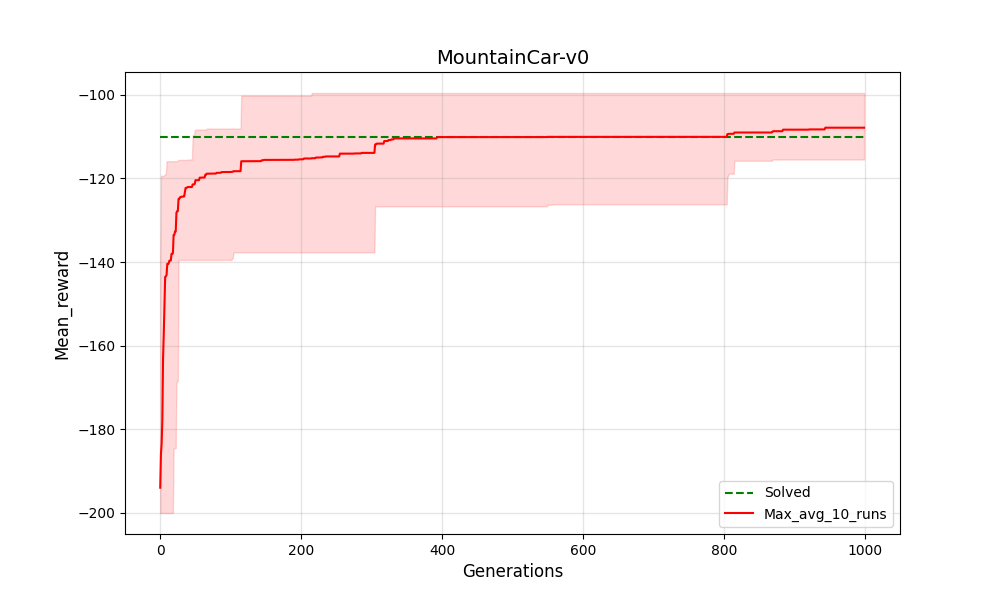
\includegraphics[width=1\linewidth]{images/MountainCar/MountainCar10run.png}
    \caption{Total training mean reward with orthogonal decision trees in the MountainCar-v0 environment, using both GE and PPO}
    \label{fig:MountainCarMean}
\end{figure}

\newpage

\begin{figure}[h!]
    \centering
    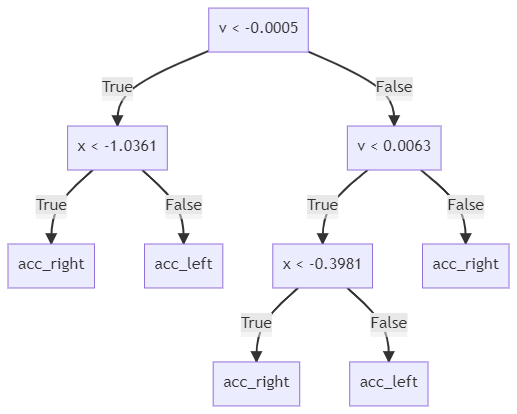
\includegraphics[width=0.5\linewidth]{images/MountainCar/bestPPOprunedMC.png}
    \caption{The best tree optimized by PPO in MountainCar-v0 environment, pruned by eliminating unnecessary branches}
    \label{fig:BestTreeMC}
\end{figure}

\newpage

\begin{figure}[h!]
    \centering
    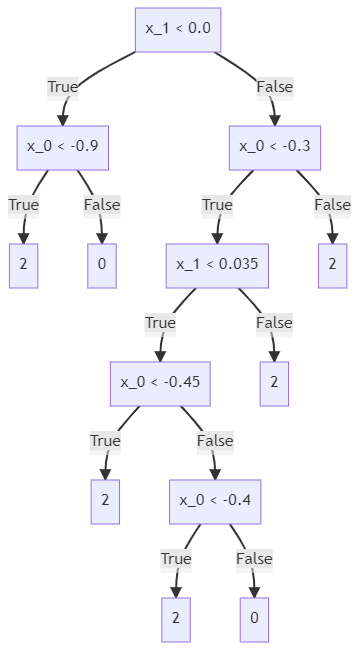
\includegraphics[width=0.4\linewidth]{images/MountainCar/bestLLCMC.png}
    \caption{The best tree obtained by L.L.Custode and G. Iacca in \cite{custode} in MountainCar-v0 environment}
    \label{fig:BestTreeLLCMC}
\end{figure}





\section{Interpretability study}
\label{sec:440}
All the obtained models are extremely easy to interpret, since they are all orthogonal DTs. Thus to determine the output given a particular state, it's necessary to check every time a Boolean condition and follow the branch accordingly until you reach a leaf where there's simply the action to take.

In the following sections, we evaluate the interpretability and the related measure of complexity, following the metric explained in Section \ref{sec:250}, of the best tree obtained via PPO for each environment.

\textit{Note:} having used oblique DTs (in which the split is composed of a linear combination of the input features and generates an oblique hyperplane) would have complicated a little the interpretability study, but would have also increased the performance of the models while still leading to more interpretable models than a neural network, as shown in \cite{custode}.

\subsection{CartPole-v1}
\label{subsec:441}
Looking at the model shown in Figure \ref{fig:BestTreeCP}, it's really easy to understand why the agent takes a decision in a particular state: 
\begin{itemize}
    \item the cart moves to the right when \[\theta < 0.0154 \land \omega > 0.2290\] or \[\theta > 0.0154\]
    \item the cart moves to the left o/w
\end{itemize}
The model, tested on 100 unseen episodes, obtained an $\mathcal{M}=35.60$, which is the same of the best tree obtained for CartPole-v1 in \cite{custode} (for the orthogonal DT).



\subsection{Acrobot-v1}
\label{subsec:442}
Looking now at the model in Figure \ref{fig:BestTreeAB} it's easy to say that:
\begin{itemize}
    \item torque +1 is applied when \[\omega_2 > 0.3094 \land \omega_1 > -2.9144\]
    \item torque -1 is applied when \[-14.2778 < \omega_2 < 0.3094 \land \omega_1 > -2.9144\] or \[\omega_2 < -14.2778\]
    \item torque 0 (do nothing) is applied o/w
\end{itemize}
The model, tested on 100 unseen episodes, obtained an $\mathcal{M}=53.4$, which is the same of the one obtained for the CartPole-v1 environment; in fact the tree has the same amount of decision nodes, but has a different structure (this type of tree is called \textit{Rule List}, like the one obtained in \cite{silva} for the LunarLander-v2 environment).


\subsection{MountainCar-v1}
\label{subsec:443}
Lastly, looking at the model in Figure \ref{fig:BestTreeMC}:
\begin{itemize}
    \item acceleration to the left is applied when \[ -0.0005 < \textit{v} < 0.0063 \land \textit{x} > -0.3981\] or \[\textit{v} < -0.0005 \land \textit{x} > -1.0361\]
    \item acceleration to the right is applied o/w
\end{itemize}
The model, tested on 100 unseen episodes, obtained an $\mathcal{M}=71.2$, which is higher w.r.t the ones obtained for the previous environments: this is because MountainCar is a more complex task compared with CartPole and Acrobot and need a more structured DT to be solved; in fact, in the configuration, it was specified that the maximum genotype length is 1024 (it was 100 for CartPole and Acrobot) and this leads to the possibility to obtain a more complex DT.

\newpage
      \emptypage
      \chapter{Final considerations and Conclusion}
\label{cha:500}
In this chapter I make the point on the aspects that could be developed further and I give some ideas for a continuous research on this.


\section{General considerations}
\label{sec:510}
In general, during all the testing process, PPO helped the max fitness to reach the solved threshold (in some environment more than others), even if it's not really connected to the evolutionary process, because of the considerations made in Section \ref{sec:330}. This work, for this reason, considered only the max fitness obtained by the best individual as metric and leave out the mean fitness of the population, due to the fact that the mean fitness is not influenced by the optimization via PPO, but it depends only on GE and for which there are already many studies about.

Despite this, PPO could also find a new state-of-the-art policy when the task had already been solved and due to this it was applied also for environment like Acrobot-v1 in which the evolutionary process converges the max fitness very quickly towards the solved threshold.

In addition, the algorithm proposed was a novel approach for which there's a very limited literature and the research is still proceeding, a fact that has stimulated myself to try to contribute, even a bit, to this cause, confirming that this is the right direction to take for AI. This fact has also led to greater difficulty to find parameters for the algorithms (and it is well-known that in AI and RL they greatly affect performance) and emboldened me to carry out a personal search of the parameters themselves, with all the consequences that ensued, such as a lower performance or a longer convergence time (in terms of generations).

Another point where I want to dwell is the environments selected for this work: we considered all the environments in the category "Classic Control" for OpenAIGym, excluding the ones that have a continuous action spaces (i.e. "Pendulum-v1" and "MountainCarContinuous-v0"); the remaining ones, as it was explained in the introduction section of the Chapter \ref{cha:400}, have different kind of reward: MountainCar and Acrobot have a sparse reward and during the testing phase, it was found out that the policies in environments like those could not be optimized correctly with PPO and for this reason, only for CartPole were found good results and PPO has really improved the evolutionary process.

This is an important point which corroborates the considerations made in \cite{ppo_acrobot} and in \cite{ppo_mountaincar} and it has to be considered for future works in this field.


Even though the results that I obtained are not overwhelming, I know that a more in-depth study could led to more encouraging performances of the algorithm and this work could be used as a starting point for futures research.


\section{Future studies}
\label{sec:520}
IAI models are already able to outperform NNs for a lot of tasks as demonstrated in many scientific papers such as \cite{custode} and \cite{silva} and are continuing to improve year after year with novel approaches like the one proposed in this work. This research could not cover every aspect of the approach used and all the approximations and workarounds done during the process deteriorated extremely the final performance of the algorithm. To improve the results, it could be done a deeper search for the hyperparameters used in PPO and also the PPO algorithm itself could be implemented in a more efficient way.

In addition, an implementation of the phenotype-to-genotype mapping function (or other techniques to insert back the optimized individual from PPO into the population) could transfer the benefits obtained from PPO shown in the Chapter \ref{cha:400} to the evolutionary process, making it more stable and lowering the necessary generations to train an agent with a max fitness.

\newpage
      
      
    \endgroup


    % bibliografia in formato bibtex
    %
    % aggiunta del capitolo nell'indice
    \addcontentsline{toc}{chapter}{Bibliography}
    % stile con ordinamento alfabetico in funzione degli autori
    \emptypage
    \bibliographystyle{plain}
    \bibliography{biblio}
    \emptypage
%%%%%%%%%%%%%%%%%%%%%%%%%%%%%%%%%%%%%%%%%%%%%%%%%%%%%%%%%%%%%%%%%%%%%%%%%%
%%%%%%%%%%%%%%%%%%%%%%%%%%%%%%%%%%%%%%%%%%%%%%%%%%%%%%%%%%%%%%%%%%%%%%%%%%
%% Nota
%%%%%%%%%%%%%%%%%%%%%%%%%%%%%%%%%%%%%%%%%%%%%%%%%%%%%%%%%%%%%%%%%%%%%%%%%%
%% Nella bibliografia devono essere riportati tutte le fonti consultate 
%% per lo svolgimento della tesi. La bibliografia deve essere redatta 
%% in ordine alfabetico sul cognome del primo autore. 
%% 
%% La forma della citazione bibliografica va inserita secondo la fonte utilizzata:
%% 
%% LIBRI
%% Cognome e iniziale del nome autore/autori, la data di edizione, titolo, casa editrice, eventuale numero dell’edizione. 
%% 
%% ARTICOLI DI RIVISTA
%% Cognome e iniziale del nome autore/autori, titolo articolo, titolo rivista, volume, numero, numero di pagine.
%% 
%% ARTICOLI DI CONFERENZA
%% Cognome e iniziale del nome autore/autori (anno), titolo articolo, titolo conferenza, luogo della conferenza (città e paese), date della conferenza, numero di pagine. 
%% 
%% SITOGRAFIA
%% La sitografia contiene un elenco di indirizzi Web consultati e disposti in ordine alfabetico. 
%% E’ necessario:
%%   Copiare la URL (l’indirizzo web) specifica della pagina consultata
%%   Se disponibile, indicare il cognome e nome dell’autore, il titolo ed eventuale sottotitolo del testo
%%   Se disponibile, inserire la data di ultima consultazione della risorsa (gg/mm/aaaa).    
%%%%%%%%%%%%%%%%%%%%%%%%%%%%%%%%%%%%%%%%%%%%%%%%%%%%%%%%%%%%%%%%%%%%%%%%%%
%%%%%%%%%%%%%%%%%%%%%%%%%%%%%%%%%%%%%%%%%%%%%%%%%%%%%%%%%%%%%%%%%%%%%%%%%%
    

    \titleformat{\chapter}
        {\normalfont\Huge\bfseries}{Appendix \thechapter}{1em}{}
    % sezione Allegati - opzionale
    \appendix
    \chapter{PPO Hyperparameters}
In this section are shown all the hyperparameters used for PPO algorithm depending on the different environment. All these were found by a manual tuning, so they aren't the optimal ones, but work well for the purpose of this thesis.\\Looking at the Tables below, the parameters stands for:
\begin{itemize}
    \item \textit{Max episode length}, is the maximum duration for an episode measured in timesteps
    \item \textit{Max training timesteps}, is the maximum duration of the total optimization process, after which the DT is returned to the main algorithm
    \item \textit{Update timestamp}, measures how often the optimization takes place (remember that PPO first takes data in order to evaluate in a second moment the actions and after that it applies the loss function for \textit{epochs} times)
    \item \textit{Epochs}, is the number of times that the backpropagation is done
    \item \textit{Epsilon clip parameter}, is a parameter for the surrogate clipped function in the loss function
    \item \textit{Gamma}, is the discount factor
    \item \textit{Learning rate actor/critic}, are the learning rates assigned to the actor/critic in the Actor-Critic model.
\end{itemize}

\begin{table}[h!]
\begin{center}
\begin{tabular}{ |c|c| } 
\hline
\textbf{Parameter} & \textbf{Value} \\
\hline
Max episode length & 500\\
Max training timesteps & $10^5$\\
Update timestamp & 3000\\
Epochs & 60\\
Epsilon clip parameter & 0.2\\
Gamma & 0.95\\
Learning rate actor & 0.001\\
Learning rate critic & 0.001\\
\hline
\end{tabular}
\caption{Parameters used for PPO in the CartPole-v1 environment}
\label{table:100}
\end{center}
\end{table}


\begin{table}[h!]
\begin{center}
\begin{tabular}{ |c|c| } 
\hline
\textbf{Parameter} & \textbf{Value} \\
\hline
Max episode length & 500\\
Max training timesteps & $10^5*1.5$\\
Update timestamp & 10000\\
Epochs & 15\\
Epsilon clip parameter & 0.2\\
Gamma & 0.95\\
Learning rate actor & 0.001\\
Learning rate critic & 0.001\\
\hline
\end{tabular}
\caption{Parameters used for PPO in the Acrobot-v0 environment}
\label{table:102}
\end{center}
\end{table}


\begin{table}[h!]
\begin{center}
\begin{tabular}{ |c|c| } 
\hline
\textbf{Parameter} & \textbf{Value} \\
\hline
Max episode length & 200\\
Max training timesteps & $10^5$\\
Update timestamp & 6000\\
Epochs & 20\\
Epsilon clip parameter & 0.2\\
Gamma & 0.95\\
Learning rate actor & 0.001\\
Learning rate critic & 0.001\\
\hline
\end{tabular}
\caption{Parameters used for PPO in the MountainCar-v1 environment}
\label{table:101}
\end{center}
\end{table}



\chapter{Complete Decision Trees and pruning method}
In this section are shown the complete version of the best trees before pruning them and it is also explained the pruning process.

\section{Full DTs}
\begin{figure}[h!]
    \centering
    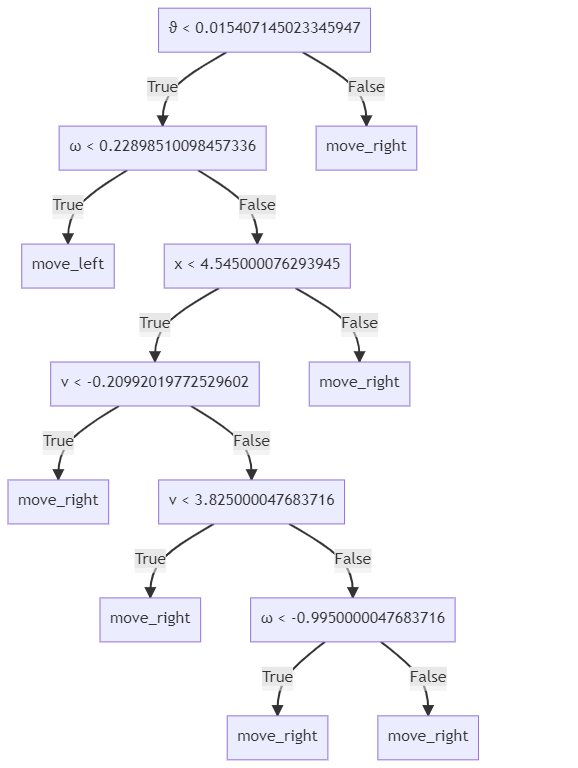
\includegraphics[width=0.7\linewidth]{images/CartPole/bestPPOcompleteCP.png}
    \caption{Full DT evolved by PPO for the CartPole-v1 environment}
    \label{fig:TreeFullCP}
\end{figure}

\begin{figure}[h!]
    \centering
    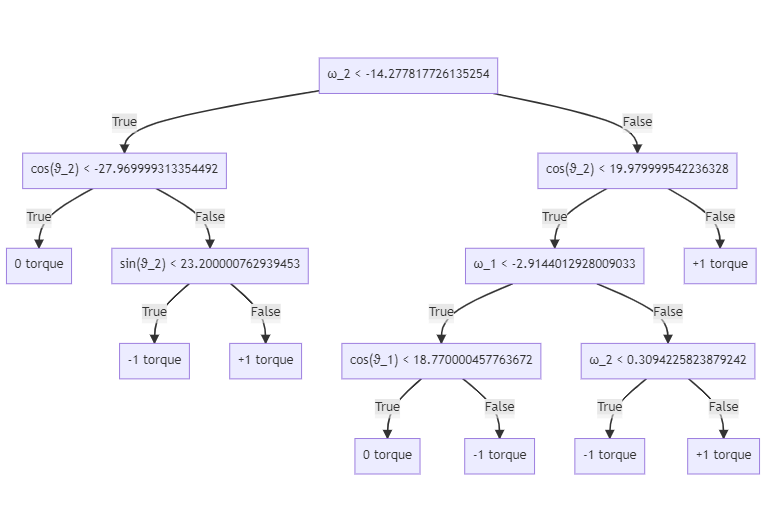
\includegraphics[width=0.7\linewidth]{images/Acrobot/bestPPOcompleteAB.png}
    \caption{Full DT evolved by PPO for the Acrobot-v1 environment}
    \label{fig:TreeFullAB}
\end{figure}

\begin{figure}[h!]
    \centering
    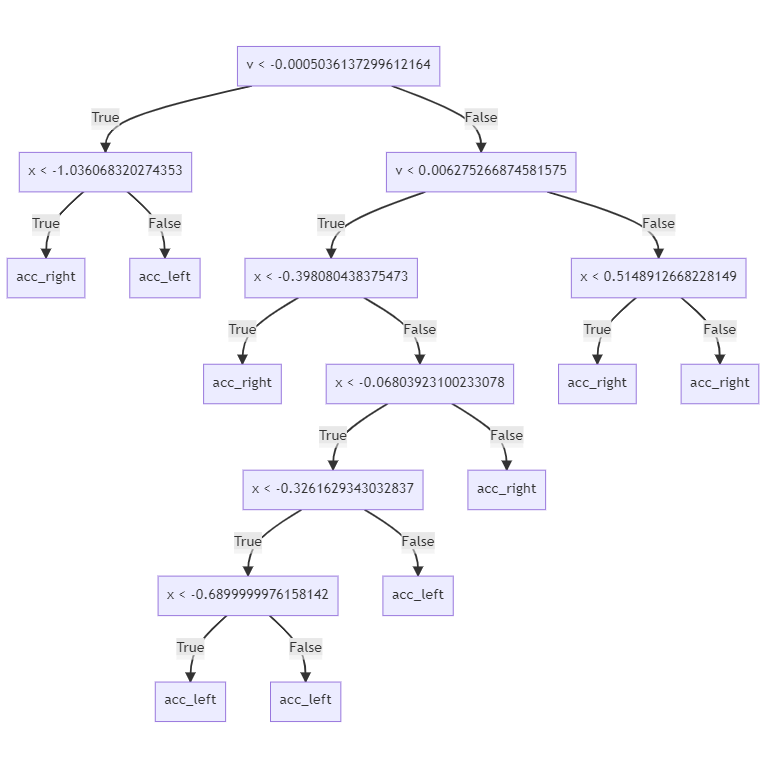
\includegraphics[width=0.7\linewidth]{images/MountainCar/bestPPOcompleteMC.png}
    \caption{Full DT evolved by PPO for the MountainCar-v0 environment}
    \label{fig:TreeFullMC}
\end{figure}

\newpage

\section{Pruning method}
\label{sec:prune}
To obtain the pruned DTs, I used a python code that tries the model in the environment for several times and marks every node that was visited. After this process, all the nodes that were not marked are eliminated and the tree is rearranged accordingly. To accentuate even more the fact that the models are highly interpretable and it's really easy and fast to prune them also by hand, I made a manual pruning of the DTs obtained in the followings subsections.

\subsection{CartPole-v1}
Considering the Figure \ref{fig:TreeFullCP} and the Subsection \ref{subsec:411} containing the constraints for the environment, starting from the root is possible to make the following considerations: the condition in the root is a valid one, so it's left untouched with its right child (a leaf). Proceeding with its left child, also this is a valid condition, so we can leave it with its left leaf. Moving now on its right child, here its possible to make a consideration to speed up the simplification process: every leaf in this subtree contains the same action, so it's possible to replace the whole subtree with a leaf containing the action in common to all the leaves (move\_right), finishing the process.

The final result is the DT shown in the Figure \ref{fig:BestTreeCP} which is quite easier to understand compared to the complete version (the split values were also rounded for a better visualization).



\subsection{Acrobot-v1}
Considering the Figure \ref{fig:TreeFullCP} and the Subsection \ref{subsec:421} containing the constraints for the environment, starting from the root is possible to make the following considerations: the root is a valid condition, so we can left it untouched.

Moving first on its left subtree, there's an invalid Boolean condition (a cosine always stands in the interval [-1,1]) and is always false: so we can connect its right subtree directly to the root; continuing on this condition, also this was pass the trigonometric boundaries and is evaluated every time as true: so we can link its left leaf to the root, removing all the conditions between, finishing the left subtree.

Proceeding on the right subtree of the root, there is a condition that is always true (passes the higher bound for cosine function): so we remove it with its right child, continuing with its left child, which is a valid condition. Despite this, its left child is an invalid condition (always true), so we can link to it the left leaf removing the condition in between. Finally, moving on its right subtree, there a valid Boolean condition.

Lastly, also the left subtree of the root is substituted with a leaf, because it's composed by a condition that lead to the same action, independently from the decision taken.

The final result is the DT shown in the Figure \ref{fig:BestTreeAB} (the split values were also rounded for a better visualization).


\subsection{MountainCar-v1}
Considering the Figure \ref{fig:TreeFullCP} and the Subsection \ref{subsec:421} containing the constraints for the environment, starting from the root is possible to make the following considerations: starting from the root, there's a valid condition, so we can leave it untouched.

Its left subtree is composed by a valid condition and 2 distinct leaves, so we can leave it untouched too.

Moving on the right subtree, we find another valid condition and also its right child is a valid condition, so there's nothing to prune here. Proceeding on the left, there's a valid condition, so it's left untouched with its left leaf. Passing on its right child, we can found a valid condition, but during the testing phases (tested on 100 unseen episode), it was found heuristically that this condition could not be false: for this reason, we can cut off it right child and connect its left subtree to its parent. Moving on the next condition, it's a valid one, so we can proceed with it's left child (the last condition); this condition is always evaluated as false due to the previous conditions: so we can remove it with its left child and connect its right leaf to its parent, finishing this process.

Lastly, we pass the tree removing all the double leaves, replacing them with its parent with a leaf containing the same action that was present in the previous leaves, concluding the pruning process.

The final result is the DT shown in the Figure \ref{fig:BestTreeMC} (the split values were also rounded for a better visualization).

\end{document}
